\documentclass[../../AISTR.tex]{subfiles}
\begin{document}
\subsection{Анализ технологического процесса}
\subsubsection{Краткое описание технологического процесса}
\paragraph{Схема}
\begin{figure}[H]
	\centering
	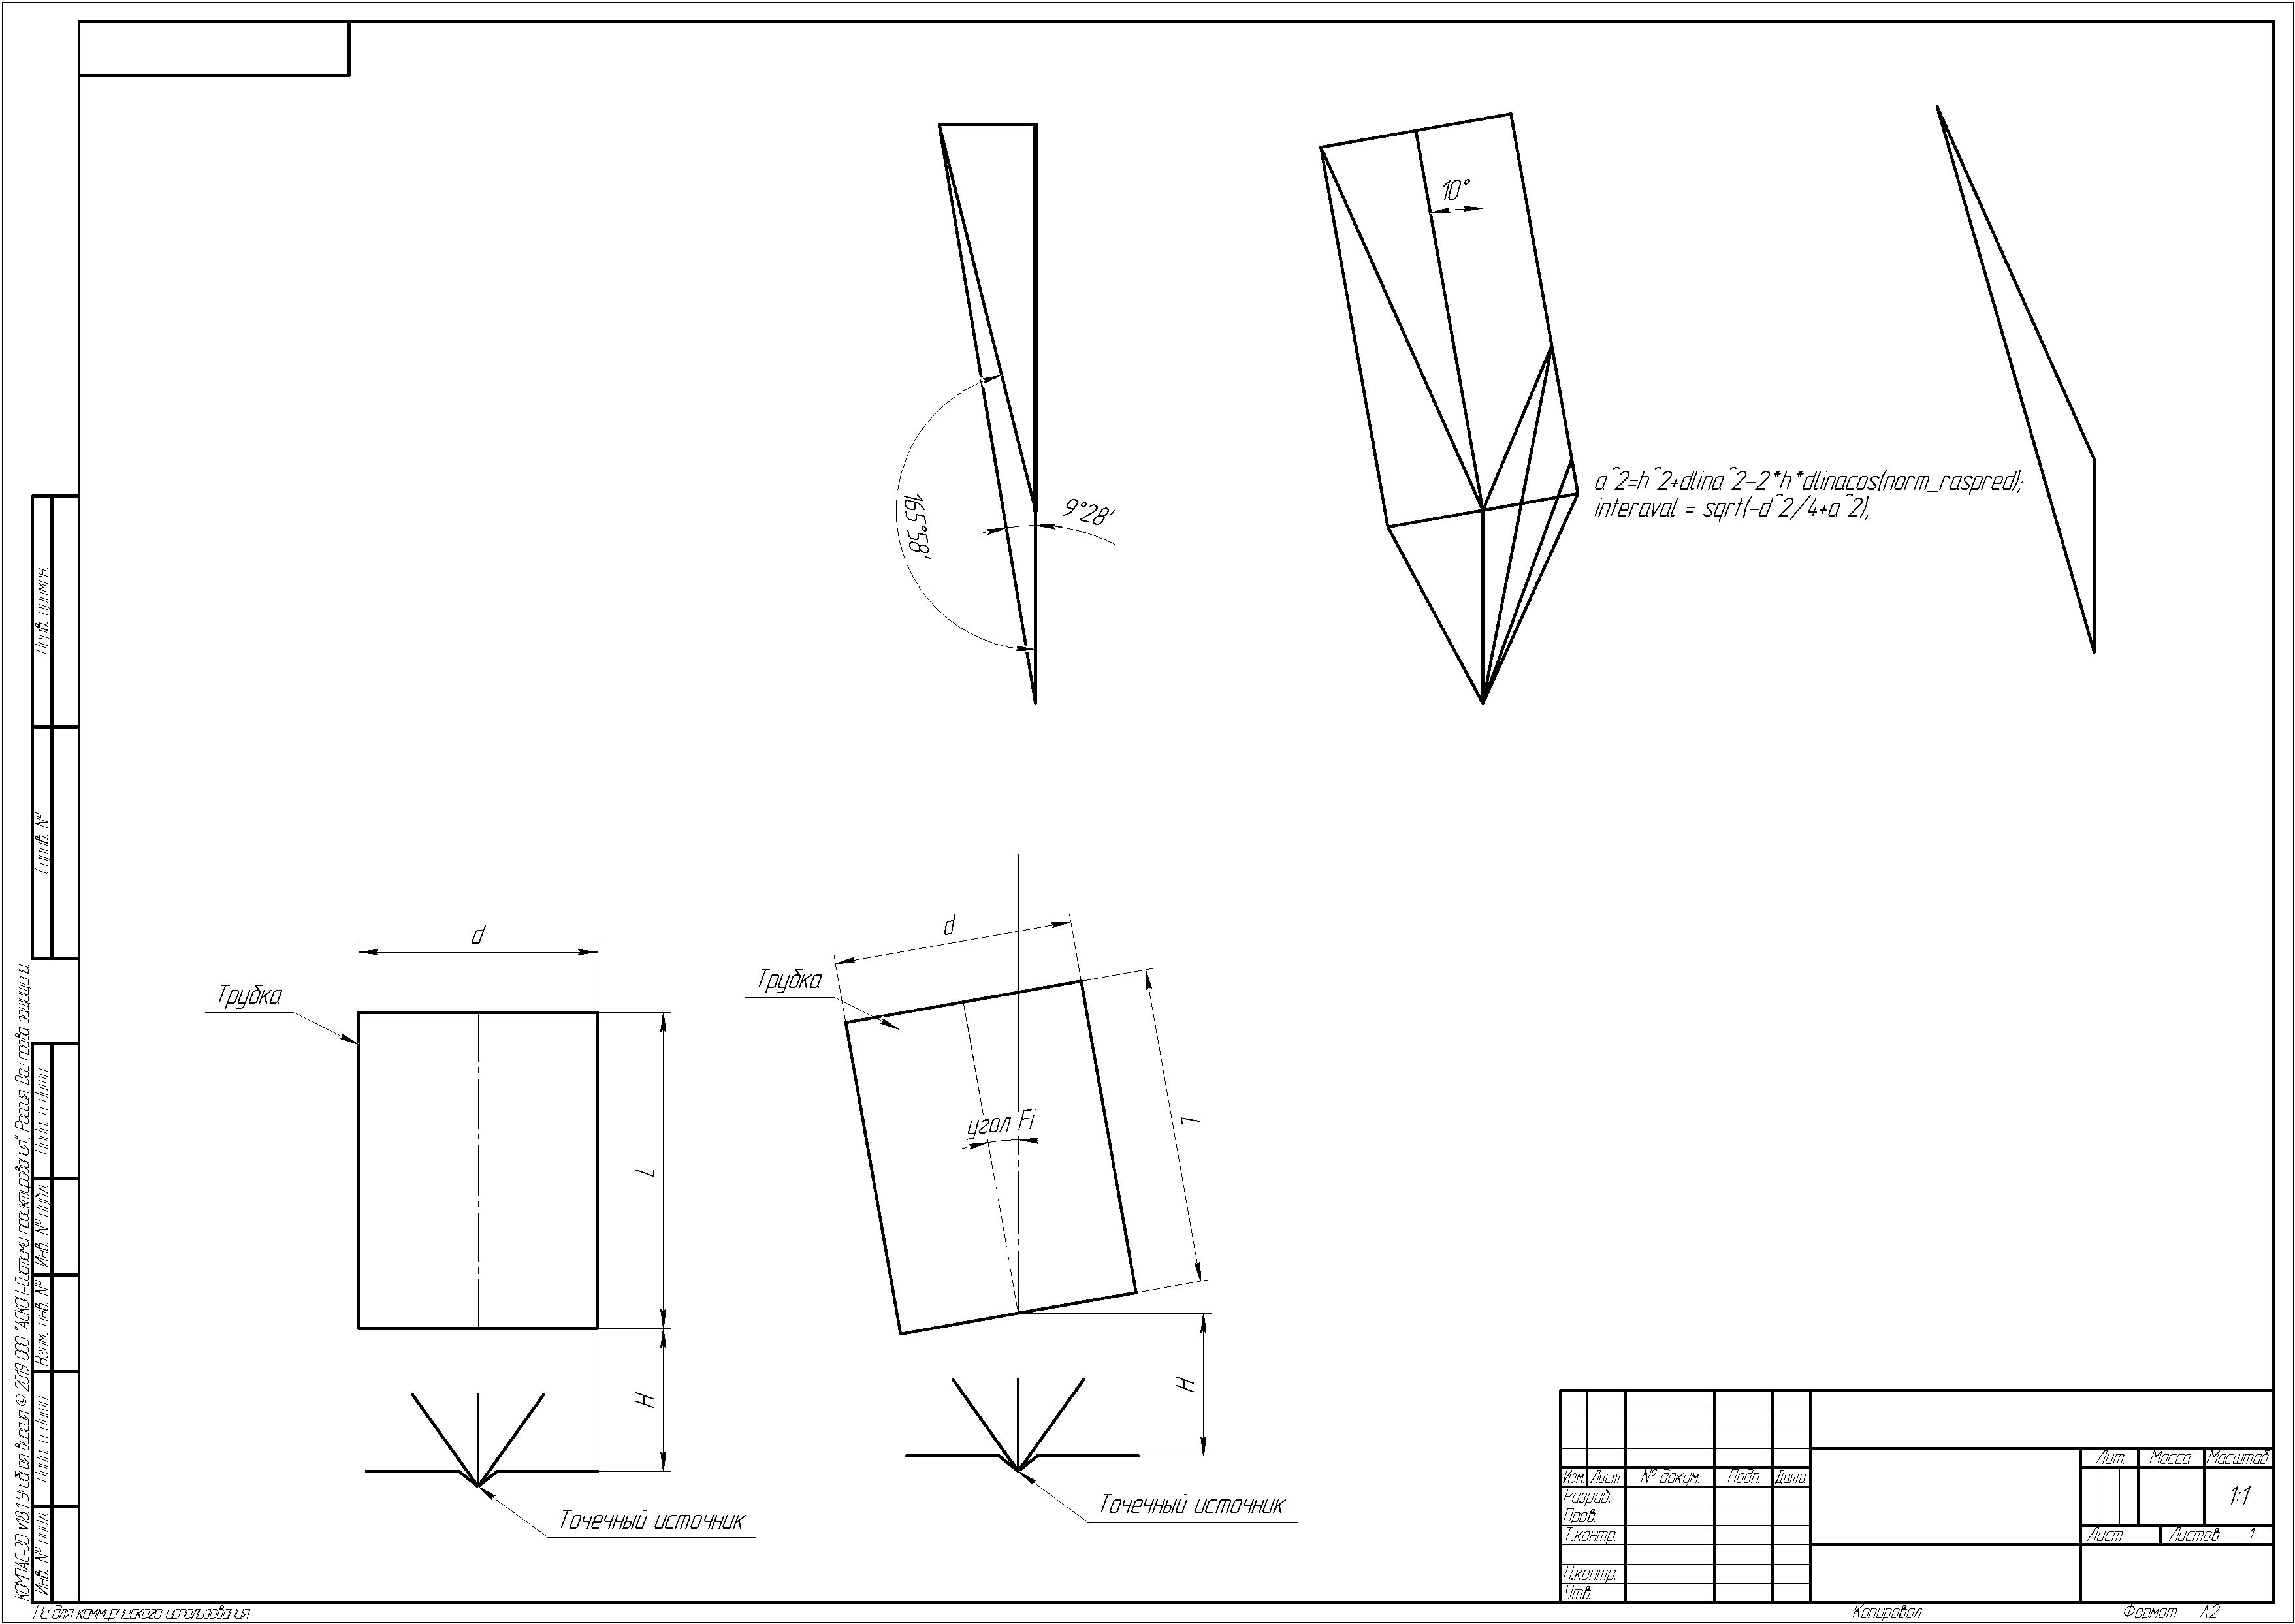
\includegraphics[trim=75 50 630 650,clip,width=0.9\linewidth]{Raschetnaya_Skhema_Dlya_Panfilovoy}
	\caption{Расчётная схема}
	\label{fig:raschetnayaskhemadlyapanfilovoy}
\end{figure}

\paragraph{Назначение процесса}
Тонкопленочные покрытия широко и многообразно применяются в различных сферах деятельности человека. В данном эксперименте на внутреннюю часть тонкой трубки наносился тонкий слой меди.
\paragraph{Сущность процесса}
Формирование тонкопленочных покрытий методом термического испарения осуществляется при сообщении материалу вещества энергии, которая затрачивается на его нагрев. С увеличением температуры колебательная энергия частиц возрастает и становится больше энергии связи с другими частицами, в результате чего происходит их испускание (испарение) и дальнейшая конденсация на поверхности изделия.

\begin{figure}[H]
	\centering
	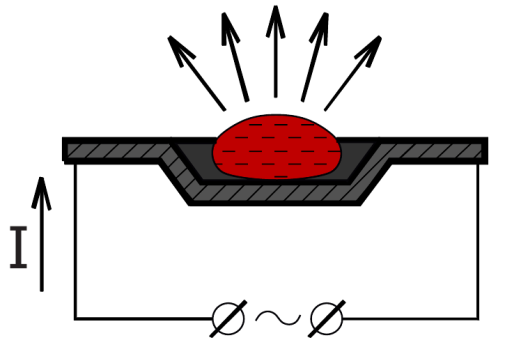
\includegraphics[width=0.5\linewidth]{resistivnoe}
	\caption{Схема резистивного термического испарения}
	\label{fig:resistivnoe}
\end{figure}


При резистивном испарении материал помещается в проводник с высоким электрическим сопротивлением (испаритель). При протекании тока через испаритель происходит его нагрев и передача тепла испаряемому веществу.
\paragraph{Этапы}
\subparagraph{При моделировании эксперимента}
\begin{enumerate}
	\item Ввод необходимых параметров в исходный код программы;
	\item Компиляция и запуск исполняемого файла;
	\item Получение результатов в виде текстового файла.
\end{enumerate}
\subparagraph{При проведении эксперимента на практике}
\begin{enumerate}
	\item Подготовка заготовки:
	\begin{itemize}
		\item Резка исходной трубы на трубы заданных параметров.
	\end{itemize}
	 \item Очистка заготовки.
	 \item Нанесение медного покрытия:
	 \begin{enumerate}
	 	\item Установка трубки в держатель;
	 	\item Откачка газа из камеры;
	 	\item Установка параметров для термического испарения;
	 	\item Нанесение покрытия;
	 	\item Остановка насосов, напуск атмосферы;
	 	\item Изъятие заготовки из камеры.
	 \end{enumerate}
\end{enumerate}
\paragraph{Используемое оборудование}
Эксперименты проводились в рамках НИР в лаборатории кафедры <<Электронные технологии в машиностроении>>. Процесс нанесения покрытия был реализован при помощи специально разработанного программного обеспечения, моделирующее нанесение покрытия методом магнетронного распыления.
\subsubsection{Сравнительный анализ входных и выходных параметров, присущих данной операции}
\begin{enumerate}
	\item \textbf{Входные контролируемые и управляемые факторы:}
	\begin{itemize}
		\item Расстояние от источника до заготовки;
		\item Время нанесения;
		\item Угол наклона заготовки относительно источника;
		\item Внутренний диаметр трубки.
	\end{itemize}	
	\item \textbf{Входные контролируемые и неуправляемые:}
	\begin{itemize}
		\item Чистота заготовки;
		\item Чистота распыляемого материала.
	\end{itemize}
	\item \textbf{Входные неконтролируемые и неуправляемые:}
	\begin{itemize}
		\item Квалификация оператора;
		\item Состояние оператора;
		\item Калибровка и настройка инструментов измерения.
	\end{itemize}
	\item \textbf{Выходные параметры:}\label{par:y}
	\begin{itemize}
		\item Отношение толщин нанесённого покрытия на противолежащих сторонах стенки (отношение толщины на левой проекции к толщине покрытия на правой).
	\end{itemize}	
\end{enumerate}

\begin{figure}[H]
	\centering
	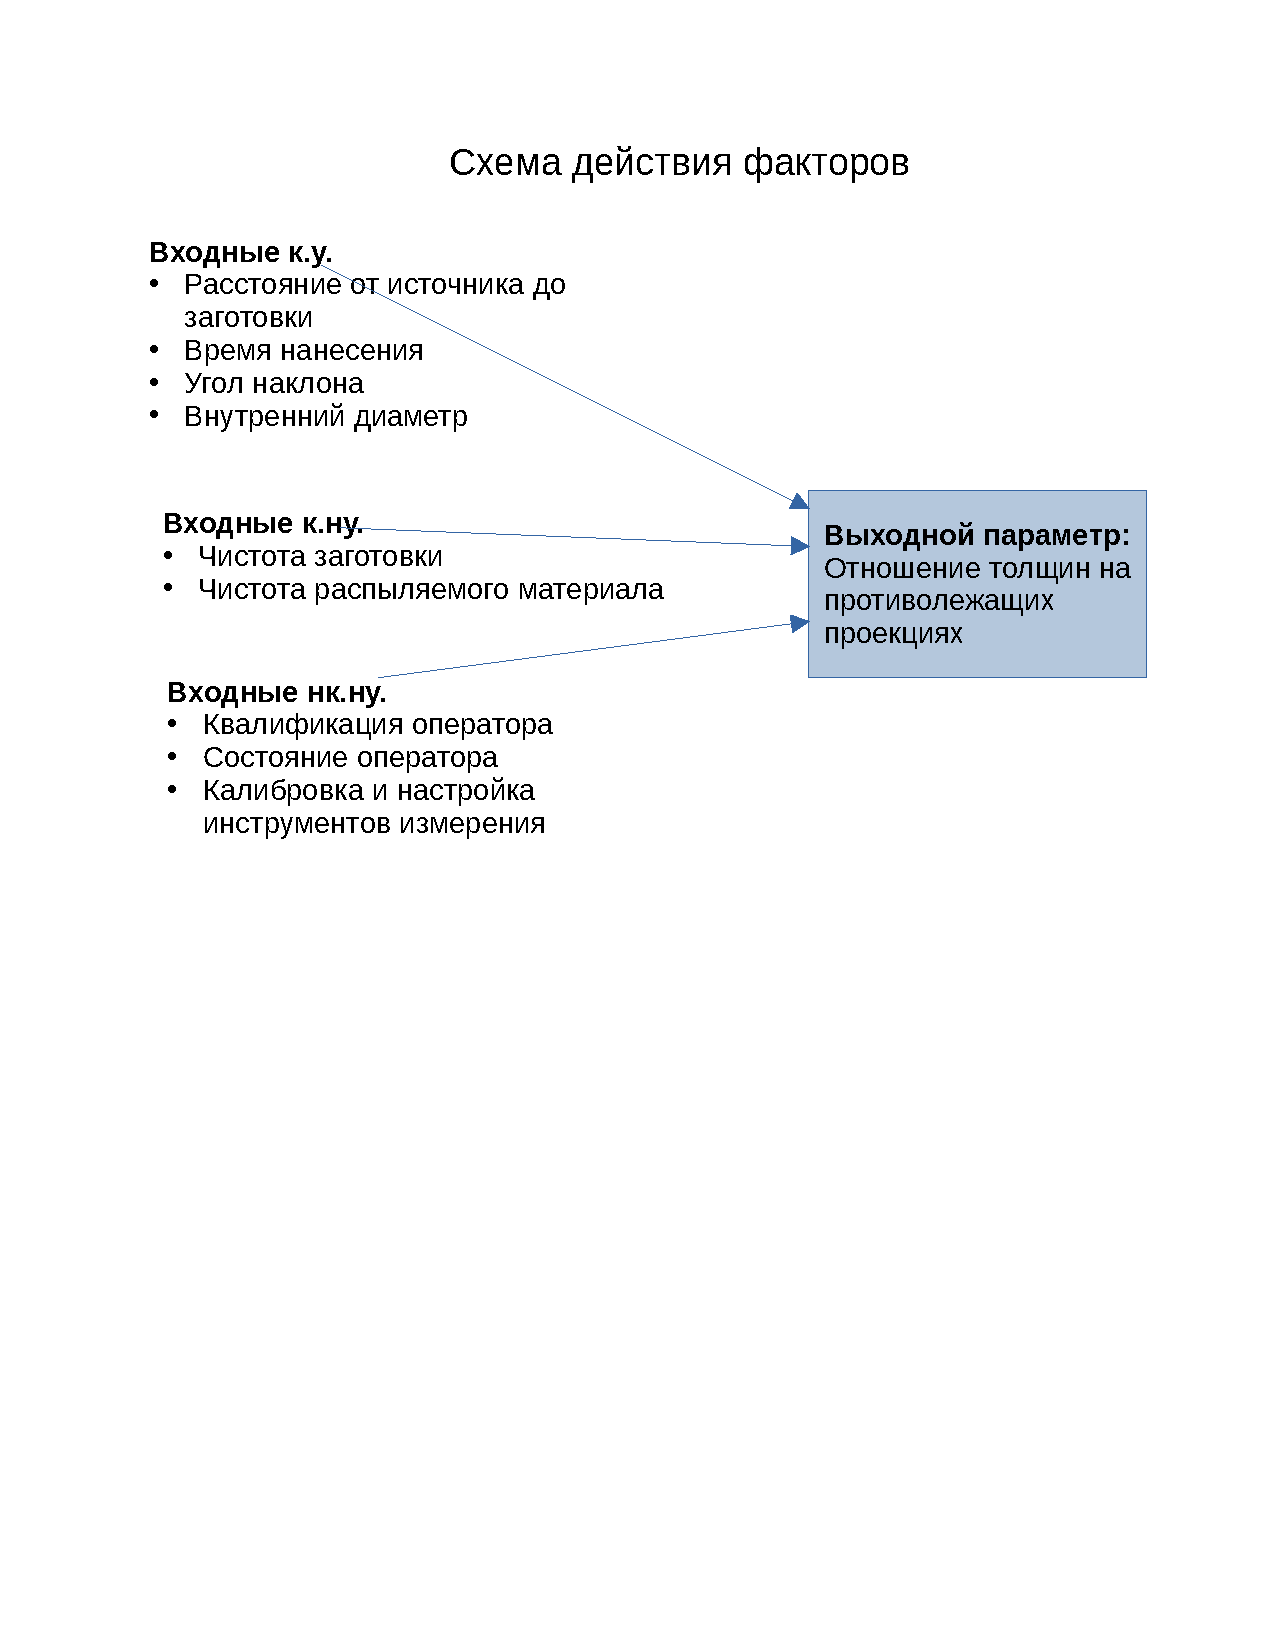
\includegraphics[trim=60 370 60 110,clip,width=0.8\linewidth]{scheme}
	\caption{Схема действия факторов}
	\label{fig:sheme}
\end{figure}


\subsubsection{Выбор наиболее существенных входных и выходных параметров}
\paragraph{Входные параметры}\label{par:vhod}
Поскольку задачей эксперимента является нахождение зависимости отношение толщин (\rbf{par:y}) напылённого материала от диаметра трубки и угла её наклона относительно источника, в качестве входных параметров были выбраны:
\begin{itemize}
	\item Диаметр трубки;
	\item Угол наклона оси трубки относительно нормали к источнику.
\end{itemize}
\paragraph{Выходные параметры}\label{par:vihod}
Из-за наклона трубки толщина покрытия на противоположных сторонах будет отличаться, в связи с чем предлагается в качестве выходного параметра взять:
\begin{itemize}
	\item Отношение толщин покрытий на противоположных стенках (какую долю от толщины покрытия на правой стороне составляет толщина покрытия на левой).
\end{itemize}
\subsection{Построение схемы контроля}
Моделирование будет производиться на компьютере и контроль будет осуществляться на нём. 
\begin{enumerate}
	\item Цилиндр высотой $L$ разделяется на 10 равных участков, считается число попавших атомов;
	\item Вычисляется средняя толщина покрытия на участке по формуле:
	\begin{equation}
		\delta = \frac{a\cdot d}{\frac{L}{10}}\whr
	\end{equation}
	\begin{itemize}
		\item $a$ -- количество попавших в данный интервал молекул;
		\item $\frac{L}{10}$ -- длина данного интервала.
	\end{itemize}
\end{enumerate}
\subsection{Проведение	математического	моделирования	технологического процесса}
\subsubsection{Обоснование необходимости проведения процесса}
Основной целью проведения эксперимента является разработка математической модели, адекватно описывающей влияние параметров процесса нанесения покрытий ITO на значение коэффициента отражения. Проведение моделирования выбранного процесса необходимо для того, чтобы определить какие из входных факторов наиболее существенно влияют на выходной параметр, а какие влияют на выходной параметр в меньшей степени. Математическое описание процесса, обычно, представляется в виде полинома:
\begin{equation}
	Y=b_0+\sum\limits_{j=1}^{k}b_jX_j+\sum\limits_{j\ne u}^{k}b_{ju}X_jX_l+\sum\limits_{j=1}^kb_jX_j^2+\ldots\whr
\end{equation}
\begin{itemize}
	\item $X$ -- факторы эксперимента;
	\item $Y$ -- функция отклика.
\end{itemize}
\subsubsection{Разработка плана эксперимента}
\begin{enumerate}
	\item В качестве метода исследования процесса выбран полный факторный эксперимент (ПФЭ). В этом случае учитывается влияние на функцию отклика исследуемого процесса не только каждого рассматриваемого в эксперименте фактора в отдельности, но и их взаимодействий.
	\item Планирование эксперимента начнём с предположения 	о том, что модель имеет вид полинома первого порядка:
	\begin{equation}
		Y=b_0+\sum\limits_{j=1}^{k}b_jX_j+\sum\limits_{j\ne u}^{k}b_{ju}X_jX_l
	\end{equation}
	\item Определение числа опытов:
	\begin{equation}
		N = u^k=(1+1)^{2}=4\whr
	\end{equation}
	\begin{itemize}
		\item $u$ -- число, на единицу большее порядка полинома
		\item $k$ -- число исследуемых факторов
	\end{itemize}
	\item Для линейной модели и 2 факторов достаточно будет провести 4 опыта, модель будет иметь вид:
	\begin{equation}\label{eq:polinom}
		Y=b_0+b_1X_1+b_2X_2+b_{12}X_1X_2\whr
	\end{equation}
	\begin{itemize}
		\item $b_0$ -- значение функции отклика в центре плана;
		\item $b_1, b_2$ -- характеристика степени влияния соответствующих факторов на функцию отклика;
		\item $b_{12}$ -- характеристика влияния взаимодействия факторов.
	\end{itemize}

\begin{figure}[H]
	\centering
	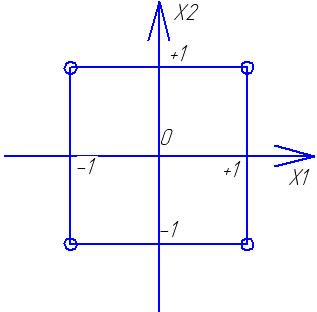
\includegraphics[width=0.3\linewidth]{plan}
	\caption{Геометрическое изображение экспериментальных точек ПФЭ}
	\label{fig:plan}
\end{figure}
\item Были выбраны следующие диапазоны варьирования факторов:

\begin{table}[H]\label{tab:diapazon}
	\centering
	\begin{tabular}{|l|C{4cm}|c|C{5cm}|}
	\hline
	Уровень & Угол наклона оси трубки,град & Диаметр трубки, мм & В безразмерной системе координат\\
	\hline
	Верхний & $6$ & $30$ & $+1$ \\
	\hline
	Нижний & $4$ & $20$ & $-1$ \\
	\hline
\end{tabular}
\caption{Диапазоны варьирования входных факторов}
\end{table}
	\item В качестве центра плана принимается центр исследуемой области. Значения входных параметров в центре плана:
	\begin{itemize}
		\item Угол наклона оси трубки $\phi=5\grad$;
		\item Диаметр трубки $d = 25$ мм.
	\end{itemize}
	\item Выходной параметр по \rbf{par:vihod} измеряется в процентах.
\end{enumerate}
\subsubsection{Построение математической модели}
Матрица планирования эксперименты имеет вид:
\begin{landscape}
	\begin{table}[H]
		\centering
		\begin{tabular}{|c|c|c|c|c|c|c|c|c|c|c|c|c|c|c|c|c|c|c|}
			\hline
			\textnumero & $x_1$&$x_2$&$X_0$&$X_1$&$X_2$&$X_1X_2$&$Y_1$&$Y_2$&$Y_3$&$Y_4$&$Y_5$&$Y_6$&$Y_7$&$Y_8$&$Y_9$&$Y_{10}$&$\bar{Y}_i$&$S_i^2$\\
			\hline
			$1$& $4$&	$20$&	$1$&	$-1$	&$-1$&	$1$&	$86.17$	&$84.34$&	$82.82$&	$80.43$&$	75.6$&	$75.52$&	$74.92$&	$74.8$&$	75.35$&	$75.53$&	$78.55$	&$19.75$
			\\
			\hline
			$2$&	$6$&	$20$&	$1$&	$1$&	$-1$&$	-1$&	$78.66$&	$71.49$&	$70.17$&	$68.43$&	$65.82$&	$65.12$&	$66.66$	&$64.85$&	$65.85$&	$66.02$&	$68.31$&	$18.12$
			\\
			\hline
			$3$&	$4$&	$30$&$	1$&	$-1$&	$1$	&$-1$	&$88.3$&	$86.75$&	$85.26$&	$82.65$&	$82.31$&	$82.13$&	$82.08$&	$82.62$&	$82.14$&	$82.79$	&$83.7$&	$5.05$
			\\
			\hline
			$4$	&$6$&	$30$	&$1$&	$1$&	$1$&	$1$&	$82.83$&	$78.04$&	$75.93$&	$75$	&$74.52$&	$74.92$&	$73.99$&	$74.5$&	$74.01$&	$74.86$&	$75.86$&	$7.39$
			\\
			\hline			
		\end{tabular}
	\caption{Матрица планирования ПФЭ}
	\end{table}

\begin{table}[H]
	\centering
	\begin{tabular}{|c|c|c|c|c|c|c|c|c|c|c|c|c|c|c|c|c|c|c|}
		\hline
		\textnumero & $x_1$&$x_2$&$X_0$&$X_1$&$X_2$&$X_1X_2$&$Y_1$&$Y_2$&$Y_3$&$Y_4$&$Y_5$&$Y_6$&$Y_7$&$Y_8$&$Y_9$&$Y_{10}$&$\bar{Y}_i$&$S_i^2$\\
		\hline
		$5$& $6$&	$27.5$&	$1$&	$1$	&$0.5$&	$0.5$&	$81.01$	&$76.09$&	$74.10$&	$72.98$&$	73.33$&	$72.34$&	$72.81$&	$72.11$&$	73.02$&	$73.14$&	$74.09$	&$7.15$
		\\
		\hline			
	\end{tabular}
	\caption{Дополнительный опыт для определения дисперсии адекватности}
	\label{tab:adek}
\end{table}
\end{landscape}
Для исключения влияния систематических погрешностей эксперимент проводился в случайном порядке.
\subsubsection{Обработка результатов эксперимента}
\paragraph{Выборочное среднее и дисперсия}
Поскольку в каждом опыте было проведено 10 параллельных наблюдений (отношение толщин на десяти интервалах), определим:
\begin{enumerate}
	\item \textbf{Выборочное среднее:}
	\begin{equation}
		\bar{Y}_i=\frac{\sum\limits_{l=1}^n Y_{il}}{n}
	\end{equation}
	\item \textbf{Выборочная дисперсия} (число степеней свободы определяется число параллельных наблюдений в каждом опыте):
	\begin{equation}
		S_i^2=\sum\limits_{l=1}^n\frac{\left(Y_{il}-\bar{Y}_i\right)^2}{n-1}
	\end{equation}
\end{enumerate}
\paragraph{Проверка эксперимента на воспроизводимость}
Проверку на воспроизводимость определим по критерию Кохрена:
\begin{enumerate}
	\item \textbf{Экспериментальное значение критерия Кохрена:}
	\begin{equation}
		G\rt{э} = \frac{\max(S_i^2)}{\sum\limits_{i=1}^N S_i^2}=\frac{19.75}{19.75+18.12+5.05+7.39}=0.39
	\end{equation}
	\item \textbf{Критическое значение критерия Кохрена:}
	\begin{equation}
		G\rt{кр} = G(\beta=0.05, N=4, n=10)=0.5\whr
	\end{equation}
	\begin{itemize}
		\item $\beta$ -- уровень значимости;
		\item $N$ -- число проведённых опытов;
		\item $n$ -- число параллельных наблюдений.
	\end{itemize}
	\item \textbf{Сравнение экспериментального и критического:}
	\begin{equation}
		G\rt{э} < G\rt{кр}
	\end{equation}
Таким образом дисперсии являются однородными, а эксперимент -- вопроизводимым.
\end{enumerate}
\paragraph{Определение коэффициентов полинома}
Коэффициенты полинома вычисляются по формуле:
\begin{equation}
	b_j = \frac{\sum\limits_{i=1}^N X_{ji}\bar{Y}_i}{N}
\end{equation}
\begin{table}[H]\label{tab:b}
\centering
\begin{tabular}{|c|c|c|c|}
	\hline
	$b_0$ &$ b_1$ & $b_2$ & $b_{12}$ \\
	\hline
	$76.61$ & $-4.52$ & $3.18$ &$ 0.60$ \\
	\hline
\end{tabular}
\caption{Значения коэффициентов полинома}
\end{table}
\paragraph{Оценка значимости коэффициентов}\label{par:znach}
Незначимость коэффициента может быть вызвана следующими причинами:
\begin{itemize}
	\item интервал варьирования соответствующей переменной мал,;
	\item уровень базового режима по данной переменной близок к точке частного экстремума;
	\item данный фактор не влияет на функцию отклика.
\end{itemize}
Проведём оценку значимости коэффициентов:
\begin{enumerate}
	\item \textbf{Дисперсия воспроизводимости} $\big($(среднее арифметическое группы выборочных дисперсий (т.е. дисперсий функции отклика по каждому
	опыту)$\big)$:
	\begin{equation}\label{eq:s_vospr}
		S^2(Y) = \frac{\sum\limits_{i=1}^N S^2_i}{N}=12.57
	\end{equation}
	\item \textbf{Дисперсия ошибки определения коэффициента}:
	\begin{equation}
		S^2\left(b_j\right)=\frac{S^2(Y)}{nN}=\frac{12.57}{10\cdot4}=0.31
	\end{equation}
	\item \textbf{Оценка значимости по критерию Стьюдента}, значение
которого рассчитывается по формуле:
\begin{equation}
	t_j = \frac{\left|b_j-0\right|}{\sqrt{S^2\left(b_j\right)}}
\end{equation}
	\item  \textbf{Критическое значение критерия Стьюдента}:
	\begin{equation}
		t\rt{кр} = t\left(\beta=0.05, \nu=N\left(n-1\right)\right)=t(0.05, 36)=2.03
	\end{equation}
	\item \textbf{Отбрасывание незначимых коэффициентов}:\label{koeff}
	\begin{table}[H]
		\centering
		\begin{tabular}{|c|c|c|c|c|}
			\hline
			&$b_0$&$b_1$&$b_2$&$b_{12}$\\
			\hline
			$t_j$ & $243.67$ & $14.38$&$10.11$&$1.91$\\
			\hline
			$t\rt{кр}$&$2.03$&$2.03$&$2.03$&$2.03$\\
			\hline
		\end{tabular}
	\caption{Критерий Стьюдента}
	\label{tab:student}
	\end{table}
Из табл. \rbf{tab:student} отбрасываем $b_{12}$ как незначимый. 
	\item \textbf{Окончательный вид модели}. Из \eqref{eq:polinom} и табл. \rbf{tab:student}:
	\begin{equation}\label{eq:matmod}
		Y = 76.61-4.52X_1+3.18X_2
	\end{equation}
\end{enumerate}
\paragraph{Проверка модели на адекватность}
\begin{enumerate}
	\item Для оценки адекватности модели необходимо определить \textbf{значения функции отклика} в каждом опыте согласно математической модели \eqref{eq:matmod}.
\begin{table}[H]
	\centering
	\begin{tabular}{|c|c|c|c|}
		\hline
		$\hat{Y}_1$ & $\hat{Y}_2$ & $\hat{Y}_3$ & $\hat{Y}_4$\\
		\hline
		$77.95$&	$68.91$&	$84.30$&	$75.26$\\
		\hline
	\end{tabular}
\caption{Значения функции отклика, рассчитанные по математической модели}
\label{tab:model}
\end{table}
	\item \textbf{Дисперсия адекватности} (оценка отклонения, предсказанного моделью значения выходного параметра (функции
	отклика) от результатов эксперимента в каждой точке факторного пространства):
	\begin{equation}\label{eq:s_ad}
		S^2\rt{ад}=\frac{\sum\limits_{i=1}^N \left(\bar{Y}_i-\hat{Y}_i\right)^2}{N-\alpha\rt{зн}}n=14.38\whr
	\end{equation}
	\begin{itemize}
		\item $\alpha\rt{зн}=3$ -- число значимых коэффициентов в полиноме;
		\item $n$ -- число параллельных измерений повторений.
	\end{itemize}
	\item \textbf{Проверка на адекватность при помощи критерия Фишера}. Сравним дисперсию адекватности \eqref{eq:s_ad} с дисперсией воспроизводимости \eqref{eq:s_vospr}:
	\begin{equation}
		F\rt{э} = \frac{\max\left(S^2\rt{ад}, S^2(Y)\right)}{\min\left(S^2\rt{ад}, S^2(Y)\right)}=\frac{S^2\rt{ад}}{S^2(Y)}=\frac{14.38}{12.57}=1.14
	\end{equation}
	\item \textbf{Критическое значение критерия Фишера:}
	\begin{equation}
		F\rt{кр} = F\left(\beta, N\left(n-1\right), N-\alpha\rt{зн}\right)=F(0.05, 36,1)=4.11
	\end{equation}
	\item \textbf{Сравнение экспериментального и критического:}
	\begin{equation}
		F\rt{э}<F\rt{кр} \Rightarrow \text{ модель адекватна}
	\end{equation}
\end{enumerate}
Таким образом, полученная модель имеет вид, показанный в \eqref{eq:matmod}
\subsection{Перерасчёт с другим значением критерия Стьюдента}
\begin{enumerate}
	\item В разделе \rbf{par:znach} в п.\rbf{koeff} коэффициент, отвечающий за взаимодействие факторов был отброшен в связи с выбором уровня значимости $\beta=0.05$. Однако, если принять уровень значимости $\beta=0.1$, значения критерия Стьюдента будет:
	\begin{equation}
		t\rt{кр} = t\left(\beta=0.1, \nu=N\left(n-1\right)\right)=t(0.1, 36)=1.69
	\end{equation}
	\item Мы получим \textbf{таблицу} \rbf{tab:student} в изменённом виде:
	\begin{table}[H]
		\centering
		\begin{tabular}{|c|c|c|c|c|}
			\hline
			&$b_0$&$b_1$&$b_2$&$b_{12}$\\
			\hline
			$t_j$ & $243.67$ & $14.38$&$10.11$&$1.91$\\
			\hline
			$t\rt{кр}$&$1.69$&$1.69$&$1.69$&$1.69$\\
			\hline
		\end{tabular}
		\caption{Критерий Стьюдента с $\beta=0.1$}
		\label{tab:student1}
	\end{table}
	\item \textbf{Модель} примет вид, отличный от \eqref{eq:matmod}:
	\begin{equation}
		Y = 76.61-4.52X_1+3.18X_2+0.59X_1X_2
	\end{equation}
	\item Необходимо будет провести \textbf{дополнительный опыт}, поскольку число значимых коэффициентов $\alpha\rt{зн}$ стало равно число проведённых опытов. Предлагается провести опыт в центре плана. Результаты опыта см. в таблице \rbf{tab:adek}.
	\item Таблица \rbf{tab:model} примет вид:
	\begin{table}[H]
		\centering
		\begin{tabular}{|c|c|c|c|c|}
			\hline
			$\hat{Y}_1$ & $\hat{Y}_2$ & $\hat{Y}_3$ & $\hat{Y}_4$&$\hat{Y}_5$\\
			\hline
			$78.54$&	$68.31$&	$83.70$&	$75.86$&$73.97$\\
			\hline
		\end{tabular}
		\caption{Значения функции отклика, рассчитанные по математической модели}
		\label{tab:model1}
	\end{table}
	\item \textbf{Дисперсия адекватности:}
	\begin{equation}\label{eq:s_ad1}
		S^2\rt{ад}=\frac{\sum\limits_{i=1}^N \left(\bar{Y}_i-\hat{Y}_i\right)^2}{N-\alpha\rt{зн}}n=0.15
	\end{equation}
Дисперсия адекватности получилась меньше, чем в  \eqref{eq:s_ad}, поскольку значения выходных параметров во всех точках кроме центральной полученные по модели и по опыту совпали.
	\item \textbf{Проверка на адекватность} (проверка с дисперсией вопроизводимости \eqref{eq:s_vospr}):
	\begin{equation}
		S^2\rt{ад}<	S^2(Y) \Rightarrow \text{модель адекватна}
	\end{equation}
\end{enumerate}



\subsection{Выводы}
\subsubsection{Выводы по модели с 3 значимыми коэффициентами}
Сравнение дисперсии адекватности и дисперсии воспроизводимости показало,
что полученная математическая модель адекватно описывает процесс нанесения
покрытий на внутренюю часть трубки.

Проанализировав полученную модель, можно сделать следующие выводы:
\begin{enumerate}
	\item Угол наклона оси трубки и её диаметр влияют на отношение толщин покрытий на противолежащих стенках;
	\item Влияние фактора $1$ (угол наклона $\phi$) более значимо, чем влияние фактора $2$ (диаметр трубки $d$);
	\item Выявлено, что эффект взаимодействия двух факторов является незначимым (эффект взамодействия был бы значимым при другом значении уровня значимости).
\end{enumerate}
\subsubsection{Выводы по модели с 4 значимыми коэффициентами}
Полученная математическая модель адекватно описывает зависимость, отношения толщин на левой и правой проекции трубки. Значение дисперсии адекватности, полученной с 3 значимыми коэффициентами \eqref{eq:s_ad} получилось больше, чем в случае с 4 значимыми коэффициентами \eqref{eq:s_ad1}.

\section{Дальнейшая работа}
Дальнейшим направлением работы является усовершенствование программы обмена данными между устройствами и осуществление автоматизации оборудования по протоколу \mb \tcp, поскольку дистанционное автоматизированное управление позволяет минимизировать такие проблемы, как:
\begin{itemize}
	\item простой оборудования в связи с отсутствием оператора;
	\item уменьшение производительности в связи с необходимостью ручного управления;
	\item ухудшение качества продукции в связи с неточным следованиям инструкциям.
\end{itemize}

Результатом работы может стать создание SCADA системы для управления вакуумным оборудованием.
\end{document}
